\item A system consists of two identical cubes, each of mass \( m \), linked together by the compressed weightless spring of stiffness \( \kappa \) (Fig. 1.41). The cubes are also connected by a thread which is burned through at a certain moment. Find:
    \begin{center}
        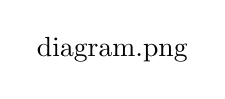
\begin{tikzpicture}
            \node at (0, 0) {{diagram.png}};
        \end{tikzpicture}
    \end{center}
    \begin{enumerate}
        \item At what values of \( \Delta l \), the initial compression of the spring, the lower cube will bounce up after the thread has been burned through.
        \item To what height \( h \) the centre of gravity of this system will rise if the initial compression of the spring \( \Delta l = \frac{7mg}{\kappa} \).
    \end{enumerate}
\begin{solution}
    \begin{center}
        \begin{tikzpicture}
            \pic at (0, 0) {frame=3cm};
        \end{tikzpicture}
    \end{center}
    
    \begin{align*}
        \intertext{The initial compression in the spring \(\Delta l\) must be such that after burning of the thread, the upper cube rises to a height that produces a tension in the spring that is at least equal to the weight of the lower cube. Actually, the spring will first go from its compressed state to its natural length and then get elongated beyond this natural length. Let \( l \) be the maximum elongation produced under these circumstances.}
        \kappa l &= mg \tag{1}
        \intertext{Now, from energy conservation,}
        \dfrac{1}{2} \kappa \Delta l^2 &= mg (\Delta l + l) + \dfrac{1}{2} \kappa l^2 \tag{2}
        \intertext{(because at maximum elongation of the spring, the speed of upper cube becomes zero).}
    \end{align*}
    \begin{align*}
        \intertext{From Eqs. (1) and (2),}
        \Delta l^2 - \dfrac{2mg \Delta l}{\kappa} - \dfrac{3mg^2}{\kappa^2} &= 0 \quad \text{or} \quad \Delta l = \dfrac{3mg}{\kappa}, \dfrac{-mg}{\kappa}
        \intertext{Therefore, acceptable solution of \(\Delta l\) equals \( \dfrac{3mg}{\kappa} \).}
        \intertext{(b) Let \( v \) be the velocity of upper cube at the position (say, at 2) when the lower block breaks off the floor, then from energy conservation,}
        \dfrac{1}{2} mv^2 &= \dfrac{1}{2} \kappa (\Delta l^2 - l^2) - mg (l + \Delta l)
        \intertext{(where \( l = \dfrac{mg}{\kappa} \) and \( \Delta l = \dfrac{7mg}{\kappa} \))}
        v^2 &= 32 \dfrac{mg^2}{\kappa} \tag{3}
        \intertext{The displacement of C.M. (of two blocks systems) in the interval in which upper block reaches position 2 is}
        \Delta y_{C_1} &= \dfrac{\left( m \cdot 0 + m (7mg/\kappa + mg/\kappa) \right)}{2m} = \dfrac{4 \, mg}{\kappa}
        \intertext{When the upper block reaches position 2, the lower block just leaves the floor with zero initial velocity. Now treat two blocks system like a single particle of mass \( 2m \) projected vertically upward with the velocity of C.M.}
        v_C &= \dfrac{mv + 0}{2m} = \dfrac{v}{2}
        \intertext{So, the further vertical displacement of C.M. of two block system}
        \Delta y_{C_2} &= \dfrac{v_C^2}{2g} = \dfrac{(v/2)^2}{2g} = \dfrac{4mg}{\kappa} \quad \text{(using Eq. 3)}
        \intertext{Hence, the net displacement of the C.M. of the system, in upward direction}
        \Delta y_C &= \Delta y_{C_1} + \Delta y_{C_2} = \dfrac{8 \, mg}{\kappa}
    \end{align*}
\end{solution}
